\documentclass[journal=jacsat,manuscript=article]{achemso}
\usepackage[version=3]{mhchem}
\usepackage{amsmath}
\newcommand*\mycommand[1]{\texttt{\emph{#1}}}
\author{Witold E. Wolski}
\author{Christian Panse}
\author{Jonas Grossman}
\author{Paolo Nanni}
\author{Ralph Schlappbach}

\abbreviations{IR,NMR,UV}

\keywords{American Chemical Society, \LaTeX}

\title[prolfqua]{Prolfqua - \textsf{Pro}teomics label free
quantification using linear models.
class\footnote{A footnote for the title}}
\makeatletter
\ifxetex
  \usepackage[setpagesize=false, % page size defined by xetex
              unicode=false, % unicode breaks when used with xetex
              xetex]{hyperref}
\else
  \usepackage[unicode=true]{hyperref}
\fi
\hypersetup{breaklinks=true,
            bookmarks=true,
            pdfauthor={},
            pdftitle={},
            colorlinks=true,
            urlcolor=blue,
            linkcolor=magenta,
            pdfborder={0 0 0}}
\urlstyle{same}  % don't use monospace font for urls

% Pandoc citation processing

% pandoc header

\begin{document}
\begin{abstract}
We introduce here the R package and benchmark linear modelling methods
available in R for label free protein expression analysis.
\end{abstract}
\begin{tocentry}
Some journals require a graphical entry for the Table of Contents.
This should be laid out ``print ready'' so that the sizing of the
text is correct.

Inside the \texttt{tocentry} environment, the font used is Helvetica
8\,pt, as required by \emph{Journal of the American Chemical
Society}.

The surrounding frame is 9\,cm by 3.5\,cm, which is the maximum
permitted for  \emph{Journal of the American Chemical Society}
graphical table of content entries. The box will not resize if the
content is too big: instead it will overflow the edge of the box.

This box and the associated title will always be printed on a
separate page at the end of the document.
\end{tocentry}

\hypertarget{introduction}{%
\section{Introduction}\label{introduction}}

The R-package for \textbf{pro}teomics \textbf{l}abel \textbf{f}ree
\textbf{qua}ntification \texttt{prolfqua} (read: prolewka) evolved from
functions and code snippets used to visualize and analyze label-free
quantification data. To compute protein fold changes among treatment
conditions, we first used t-test, linear models, or functions
implemented in the package limma. We evaluated
\href{10.18129/B9.bioc.MSstats}{MSStats},
\href{10.1038/s41598-017-05949-y}{ROPECA} or
\href{https://github.com/statOmics/MSqRob}{MSqRob} all implemented in R,
with the idea to integrate the various approaches in our analysis
pipeline. Although these packages are implemented in R, model
specification, input, and output formats differ widely and wildly.
Furthermore, to better understand the inferences produced, we decided to
use the R linear and mixed effect models directly and transparently and
to reimplement some features from the other packages when considered
useful. The R-package prolfqua is the outcome of this venture.

The \emph{prolfqua} package integrates most of the steps of the LFQ data
analysis workflow: quality control, data normalization, protein
aggregation, sample size estimation, modeling, and hypothesis testing.
For instance, the quality control module makes it easy to determine the
coefficients of variations (CV) for peptides and proteins within
conditions, summarize and visualize missing data or intensities.

When developing \emph{prolfqua}, we draw inspiration from packages such
as \emph{sf}, which uses data in a long tidy table format. We represent
the data needed for analysis using a single data-frame in long format
and an R6 configuration object. Using the configuration object, we
specify what data is in which column, making it easy to integrate new
inputs if provided in long tidy tables. All that is needed to
incorporate Spectronaut, Skyline text output, or the \textbf{MSStats}
data format is a few code lines of code to update the configuration
object. For software like MaxQuant or MSFragger, which writes the data
into a wide table, with several intensity columns, one for each sample,
we implemented methods that transform the data into a long tidy table.
Relying on the long tidy data table enabled us to easily interface with
many data manipulation, visualization, and modeling methods implemented
in base R and the \emph{tidyverse}.

R linear model and linear mixed effect models allow modeling parallel
designs, repeated measurements, factorial designs, and many more. R's
formula interface for linear models is flexible, widely used, and well
documented. We integrate R's linear model and mixed model formula
interface in \emph{prolfqua}'s API. This glass box approach should make
it easy to reimplement an analysis performed with prolfqua using base R
or other programming languages by reading the analysis script and
without looking at the package code. Knowledge of the R regression model
infrastructure is an advantage when using our package. Acknowledging the
formula interface's complexity and the popularity of MSstats, we
provided functionality to derive the model formula from an MSstats data
format.

The prolfqua package fits the linear model to all the proteins in the
dataset. Afterward, we can compute contrast to test the hypothesis,
perform ANOVA, or model selection using the likelihood ratio test for
thousands of proteins. By exploiting the parallel structure of the
analysis, \emph{prolfqua} implements t-statistic moderation to improve
inference for small sample sizes {[}\emph{limma}{]}. It also computes
probabilities of differential protein regulation based on peptide level
models {[}\emph{ropeca}{]}.

To optimize a data analysis workflow, prolfqua implements and integrates
benchmarking methods, e.g., computing ROC curves. We implemented these
methods to assess differences between linear models, mixed effect
models, p-value moderation, or Bayesian regression models using the
IonStar dataset.

We developed and improved the package by applying the ``Eating your own
dog food'' principle. We used it to analyze SRM, PRM, and LFQ data and
to generate analysis reports. The current iteration of the packages API
groups the functionality into R6 classes (e.g., LFQPlotter,
LFQSummarizer, LFQStats, Model, Contrast, etc.). We choose R6 for its
visual debugging and code completion support in RStudio.

We believe that the package makes it easy to perform proteomics
quantitative data analysis, generate visualizations, and integrate them
into reproducible reports using Rmarkdown. You can install the package
from \url{www.github.com/wolski/prolfqua}, and we are working on making
it available on Bioconductor.

\hypertarget{methods}{%
\section{Methods}\label{methods}}

\hypertarget{benchmarking}{%
\subsection{Benchmarking}\label{benchmarking}}

The benchmark dataset contains \emph{H. sapiens} proteins with constant
concentrations and \emph{E. coli} proteins with varying
concentration.\textsuperscript{\textbf{shen2018ionstar?}} We know that
for \emph{H. sapiens} proteins the difference \(\beta\) between two
dilutions should be \(\beta = 0\) while for \emph{E. coli} proteins we
know that the difference between dilutions should be \(\beta \ne 0\).

We can use various statistics to examine this hypothesis: the contrast
estimate \(\beta\), or because we first log2 transformed the data the
log2 fold-change (log2FC), the t-statistic
\(\frac{\beta}{\sqrt{var(\beta)}}\), the \(p-value\) and moderated
\(p-value\) for models where the p-value can be obtained.

For Bayesian models we can use the posterior probabilities that
\(\beta=0\), e.g.~the probability that \(\beta < 0\) when the mean
estimate \(\hat{\beta}\) is greater \(0\) or vice versa,
i.e.~\(P(\beta < 0| \hat{\beta} > 0)\) or
\(P(\beta > 0 | \hat{\beta} < 0)\), which we can compute from the
posterior sample of the \(\beta\) parameters. We can also use the
statistic \(\frac{mean(\beta)}{\sqrt{var(\beta)}}\) with \(var{\beta}\)
estimated from the posterior sample of the \(\beta\) parameter.

For each statistic and each value of the statistics we then compute a
confusion matrix (see Table @ref(tab:confusionMatrix)). From the
confusion matrix we can compute measures such as true positive rate
(TPR), false positive rate (FPR), false discovery proportion (FDP) or
accuracy (ACC) which are given by:

\begin{table}

\caption{\label{tab:confusionMatrix}Confusion matrix, TP - true positive, FP - false positive, FN - false negative, P - all positive cases (all E. coli proteins), N - all negative cases (all H. sapiens proteins), m- all proteins.}
\centering
\begin{tabular}[t]{l|l|l|l}
\hline
Prediction \textbackslash{} Truth & E.coli & H.sapiens & Total\\
\hline
beta != 0 & TP & FP & R\\
\hline
beta == 0 & FN & TN & \\
\hline
Total & P & N & m\\
\hline
\end{tabular}
\end{table}

\[
\begin{aligned}
TPR &= \frac{TP}{TP+FN} = \frac{TP}{P}\\
FPR &= \frac{FP}{FP+TN} = \frac{FP}{N}\\
FDP &= \frac{FP}{TP + FP} = \frac{FP}{R}\\
ACC &= \frac{TP + TN}{m}
\end{aligned}
\]

By plotting the \(TPR\) versus the \(FPR\) we obtain the receiver
operator characteristic curve (ROC curve). The area under the curve
(AUC) or partial areas under the curve (pAUC), at various values of the
\(FPR\), are further measures of performance. By using these measures we
can compare the performances of the statistics produced by the various
methods examined.

A further question we can examine using the benchmark data is, how well
the false discovery estimate (FDR) obtained to from the statistical
model matches the false discovery proportion (FDP). The FDR is the
expected value of the false discovery proportion. Ideally, the FDR
should be an unbiased estimate of the \(FDP\). By plotting the FDR
gainst the FDP we can asses visually if these assumptions are met.

For the Bayesian models we obtain an FDR estimate by first computing the
p-value using the statistic \(\frac{mean(\beta)}{\sqrt{var(\beta)}}\)
and assuming that it is normally distributed. We then obtain the FDR by
adjusting the p-values using the Benjamini-Hochberg procedure.

For some of the proteins, quantification results are missing in some
conditions. All we required when attempting to fit a model for a protein
is that there are at least two peptides per protein quantified in any of
the twenty samples. That means that for some proteins, not all model
parameters are estimable. In case of the linear model, the contrast
function we implemented can handle partial models and provides estimates
of some of the contrasts (see Table @ref(tab:tablesMedpolish)). For the
mixed effect models, the used \texttt{lmerTest::contest} function does
not support models with missing parameter estimates, and hence we have 4
(all) or 0 (no) contrast estimates for a protein (see Table
@ref(tab:tablesMM)). For the Bayesian models obtained with \emph{brms}
or \emph{rstan} we also only computed contrasts for models with complete
fixed effect estimates (see Tables @ref(tab:countsBrms),
@ref(tab:countsBrmsStudent) and @ref(tab:countsRstand)). The ROPECA
approach starts by fitting a model to each peptide and the contrast
function can handle missing parameter estimates (see Table
@ref(tab:tablesRopeca)). These differences result in different numbers
of fold-change estimates for each type of model, i.e.~in a different set
of ground truths, which makes comparing model performances involved. To
deal with these differences, we computed our benchmark estimates,
including the peptides and proteins, without fold-change estimates, by
accordingly updating the numbers in the confusion matrix. To compute the
\(FPR\) and \(TPR\) including the missing estimates we set \(P =\) \#all
\emph{E. coli} peptides/proteins detected, and \(N =\) \#all \emph{H.
sapiens} proteins detected.

\hypertarget{benchmark-data-preprocessing}{%
\subsection{Benchmark Data
preprocessing}\label{benchmark-data-preprocessing}}

We fitted the models using all the \(20\) samples of the IonStar dataset
(see Figure @ref(fig:ionstar)), i.e.~five different dilutions, with four
technical replicates each. This allows to estimate ten different
contrasts shown in Table @ref(tab:setupContrasts). For benchmarking we
only used the contrasts resulting in small fold-changes
\(\beta = 1.2,1.25,1.3(3),1.5\) listed in Table @ref(tab:usedContrasts).
Only those small fold-changes allowed us to see differences among the
methods. For the larger fold-changes no differences can be seen among
the models or statistics.

Data was preprocessed by \(log_2\) transforming the peptide intensities,
and subsequent robust z-score transformation. No other data filtering
was used than the removal of \emph{one hit wonders}, i.e.~proteins with
a single peptide assignment (For details see section {[}Datasets and
Data preprocessing{]}). We did not use imputation. The only differences
we will observe are because of using different modelling methods.

\[
z = \frac{x - \bar{x}}{S} \sim \frac{x - \tilde{x}}{\tilde{S}}
\] t fold change on the original scale, we multiply the z-score by the
average variance of all the \(N\) samples in the experiment.

\[
z' = z \times 1/N\sum_{i=1}^N S_i
\] We decided to apply this simple transformation because it only
requires to estimate two parameters per sample and works for experiments
with thousands of proteins as well as for experiments where only a few
hundreds of proteins per sample are measured.

\begin{verbatim}
##                                       contrastsName dilution     ratio expected fold change
## dilution_(9/3)_3                   dilution_(9/3)_3 dilution     (9/3)                    3
## dilution_(9/4.5)_2               dilution_(9/4.5)_2 dilution   (9/4.5)                    2
## dilution_(9/6)_1.5               dilution_(9/6)_1.5 dilution     (9/6)                  1.5
## dilution_(9/7.5)_1.2           dilution_(9/7.5)_1.2 dilution   (9/7.5)                  1.2
## dilution_(7.5/3)_2.5           dilution_(7.5/3)_2.5 dilution   (7.5/3)                  2.5
## dilution_(7.5/4.5)_1.6(6) dilution_(7.5/4.5)_1.6(6) dilution (7.5/4.5)               1.6(6)
## dilution_(7.5/6)_1.25         dilution_(7.5/6)_1.25 dilution   (7.5/6)                 1.25
## dilution_(6/3)_2                   dilution_(6/3)_2 dilution     (6/3)                    2
## dilution_(6/4.5)_1.3(3)     dilution_(6/4.5)_1.3(3) dilution   (6/4.5)               1.3(3)
## dilution_(4.5/3)_1.5           dilution_(4.5/3)_1.5 dilution   (4.5/3)                  1.5
##                                         contrasts
## dilution_(9/3)_3          dilution.e - dilution.a
## dilution_(9/4.5)_2        dilution.e - dilution.b
## dilution_(9/6)_1.5        dilution.e - dilution.c
## dilution_(9/7.5)_1.2      dilution.e - dilution.d
## dilution_(7.5/3)_2.5      dilution.d - dilution.a
## dilution_(7.5/4.5)_1.6(6) dilution.d - dilution.b
## dilution_(7.5/6)_1.25     dilution.d - dilution.c
## dilution_(6/3)_2          dilution.c - dilution.a
## dilution_(6/4.5)_1.3(3)   dilution.c - dilution.b
## dilution_(4.5/3)_1.5      dilution.b - dilution.a
\end{verbatim}

\begin{table}

\caption{\label{tab:usedContrasts}Contrasts used for benchmark.}
\centering
\begin{tabular}[t]{l|l|l|l}
\hline
  & contrasts & ratio & expected fold change\\
\hline
dilution\_(9/7.5)\_1.2 & dilution.e - dilution.d & (9/7.5) & 1.2\\
\hline
dilution\_(7.5/6)\_1.25 & dilution.d - dilution.c & (7.5/6) & 1.25\\
\hline
dilution\_(6/4.5)\_1.3(3) & dilution.c - dilution.b & (6/4.5) & 1.3(3)\\
\hline
dilution\_(4.5/3)\_1.5 & dilution.b - dilution.a & (4.5/3) & 1.5\\
\hline
\end{tabular}
\end{table}

Furthermore, we will only model protein fold-changes of proteins were at
least two peptides were observed. The reason is that peptide
identification has an associated error which is significantly reduced if
two independent peptide identifications of a protein are observed. Many
proteomics journals require to only report proteins identified by two
peptides. Proteins identified by only a single peptide are sometimes
called ``one-hit
wonders.''\textsuperscript{\textbf{mendoza2018flexible?}}

In order to remove systematic differences among samples, peptide
intensities need to be transformed and scaled. The transformation aims
to remove heteroscedasticity while the scaling aims to remove systematic
differences among samples. Because the size of the error is proportional
to the intensity, by \(\log\) transforming the intensities this error
can be modelled with \(\epsilon \propto N(0, \sigma^2)\).

Valikangas\textsuperscript{\textbf{valikangas2016systematic?}} and
colleagues discuss and benchmark various methods of peptide or protein
intensity normalization such as variance stabilizing
normalization\textsuperscript{\textbf{huber2002variance?}} or quantile
normalization.\textsuperscript{\textbf{bolstad2003comparison?}} In this
work we will be using a robust version of the z-score, where instead of
the mean we use the median and instead of the standard deviation the
median absolute deviation (mad):

\[
z = \frac{x - \bar{x}}{S} \sim \frac{x - \tilde{x}}{\tilde{S}}
\]

Because we need to estimate the protein fold-changes on the original
scale, we have to multiply the \(z\)-score by the average variance of
all the \(N\) samples in the experiment.

\[
z' = z \times 1/N\sum_{i=1}^N S_i
\] We decided to apply this simple transformation because it only
requires to estimate two parameters per sample and works for experiments
with thousands of proteins as well as for experiments where only a few
hundreds of proteins per sample are measured. For the Ionstar dataset we
used the intensities of \emph{H. sapiens} proteins, whose concentrations
do not change, to determine \(\bar{x}\) and \(S\) and than applied it to
all the intensities (including \emph{E. coli}) in the sample.

Figure @ref(fig:scaling) shows the distribution of the peptide
intensities within the samples before and after the intensity scaling.
Figure @ref(fig:variancestable) shows the coefficient of variation
before log transforming and scaling the data and the distribution of the
standard deviations afterwards.

(ref:scaling) Density plot of peptide intensities before (panel A) and
after (panel B) data transformation and scaling.

\begin{figure}
\centering
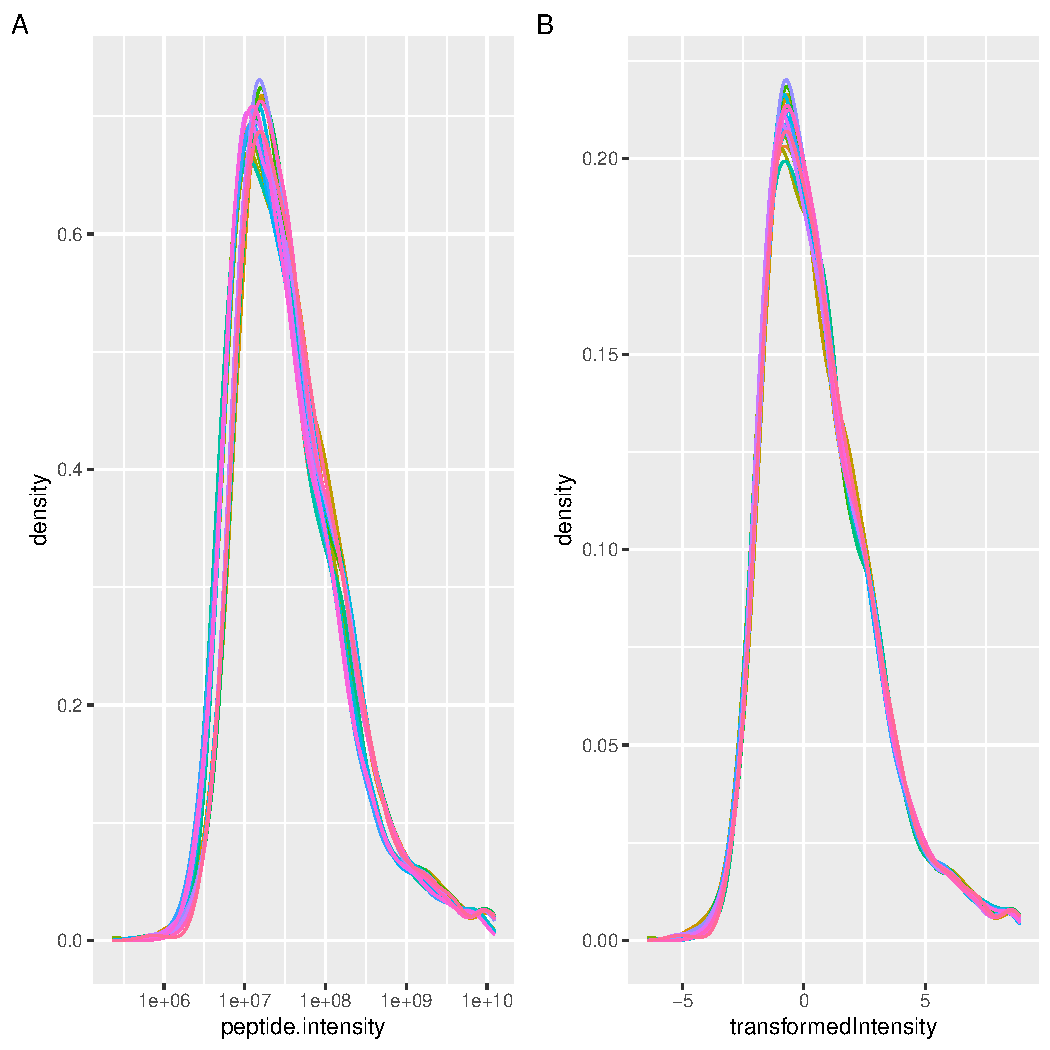
\includegraphics{Prolfqua_files/figure-latex/scaling-1.pdf}
\caption{(ref:scaling)}
\end{figure}

\hypertarget{linear-model}{%
\subsection{Linear model}\label{linear-model}}

Here we show how the two-stage modelling by first estimating the protein
intensities using the Tukey median polish and then fitting a linear
model performs.

\hypertarget{results-and-discussion}{%
\section{Results and discussion}\label{results-and-discussion}}

In this section we compare the results for the various models
implemented and discussed previously, namely:

\begin{itemize}
\tightlist
\item
  (\texttt{prot\_med\_lm}) : linear model fitted to protein estimates
  obtained using Tukey's median polish
\item
  (\texttt{prot\_lme4}) : mixed effects model fitted using \emph{lme4}
\item
  (\texttt{prot\_ROPECA}) : linear models fitted on peptide level and
  aggregation of moderated p-values using the beta distribution
\item
  (\texttt{prot\_rstan}) : mixed effects model fitted with \emph{rstan}
  and with prior over \(\varepsilon\)
\item
  (\texttt{prot\_brms}) : mixed effects model fitted with \emph{brms}
  and default priors
\item
  (\texttt{prot\_brms\_student\_t}) : mixed effects model fitted with
  \emph{brms} and shrinkage prior over fixed effects coefficients .
\end{itemize}

A relevant parameter is the number of proteins for which we estimated
the contrasts (see Table @ref(tab:completeCasesTab)). It indicates how
robust the models are in the presence of missing data. We observe, that
when using the linear model on protein level intensities or the bayesian
version of the mixed effects models we were able to estimate for 4024
(out of the 4099) proteins all the four examined contrasts (complete
cases). When using the mixed effect model implementation in \emph{lme4}
this number drops to \(4013\), while when summarizing peptide level
models it drops further to \(3999\) proteins.

The different number of proteins for which we obtained statistics of
contrasts makes comparing the scores for various models complicated
because the set of proteins differs, e.g.~\(4024\) versus \(3999\).
Therefore, we incorporate the failure to generate statistics for
contrasts into the benchmark by setting \(P\) and \(N\) equal to the
number of all proteins (see Table @ref(tab:confusionMatrix)) and then
computing the \(FPR\) and \(TPR\).

\hypertarget{outline}{%
\subsection{Outline}\label{outline}}

\hypertarget{extra-information-when-writing-jacs-communications}{%
\section{Extra information when writing JACS
Communications}\label{extra-information-when-writing-jacs-communications}}

\begin{acknowledgement}

The authors thank technology platform fund of the University of Zurich.


\end{acknowledgement}

\begin{suppinfo}

This will usually read something like: ``Experimental procedures and
characterization data for all new compounds. The class will
automatically add a sentence pointing to the information on-line:

\end{suppinfo}

\hypertarget{references}{%
\subsection{References}\label{references}}
\end{document}
